\chapter{Preliminaries}
\section{Advanced Persistent Threat}

APT stands for Advanced Persistent Threat, a kind of sophisticated attack which requires an advanced level of expertise and aims to remain persistent on the attacked infrastructure.

The term APT can refer to a persistent attack with a specific target, or it can refer to the group that organized the attack, sometimes the group is affiliated with some sovereign state.
\\

To understand better what is an APT, we need to decompose the word: 

\textbf{Advanced:} the people behind the attack have an advanced level of expertise, resources, and money. They usually do not use known malware, but they write their malware specific to the target they want. Moreover, they can gather information on the target from the intelligence of their country of origin.

\textbf{Persistent:}  The adversary does not aim to gain access in the most number of system, but rather to have persistent access to the infrastructure. The more time they remain undiscovered in the organization's network infrastructure, the higher are the chances of lateral movement, the greater are the information they can gather. Persistent access is the key to every APT.

\textbf{Threat:} As said before, this is an organized threat, with a strategical vision of what to achieve. It is not an automatic tool that attacks everything trying to gather something. It is a meticulously planned attack that aims to obtain certain information from a given organization. \cite{apt_def}
\\

In general, APTs aim to higher-value targets like other nations or some big corporations. However, any individual can be a target. FireEye publish a report each year about the new APT campaign, the diagram below states which industry is the most attacked in the last year.\\

\begin{figure}[!h]
	\centering
	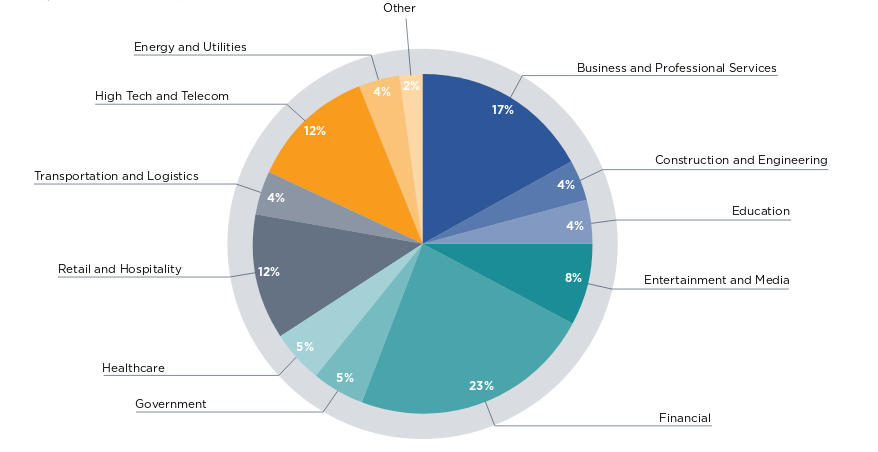
\includegraphics[width=1.0\columnwidth]{graph}
	\caption{Diagram of industry target}
\end{figure}

A point of particular concern is the retargeting, in the Americas, 63\% of the companies attacked by an APT, are attacked again last year by the same or similar group. In the Asian and Pacific areas, this is even worse, 78\% of the industries are hacked again. \cite{fireeye_mtrends} \\


\begin{figure}[ht!]
	\centering
	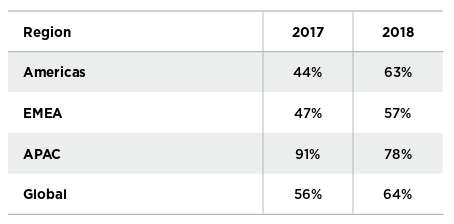
\includegraphics[width=0.5\columnwidth]{retarget}
	\caption{Retargeting divided by regions}
\end{figure}

Advanced persistent threats, contrary to regular malware, are composed of different phases, each of which has an important role. 

The attack is decomposed into smaller steps, for example, if a group of hackers wants to attack a CEO of a given company, they will not send directly to the CEO a phishing email, because it's likely that he has a complex system of security and they would be detected instantly. 

Instead, the first step would hack a person in the same company with lower permissions that can have minor defense mechanisms. Once they got the first computer, they can explore the network infrastructure of the organization, and then decide which action is the best.
They could cover their track from the log system, or locate the data they need or send a phishing email to the CEO from the owned user.\\

So how does an APT work? Fireeye described their behavior in six steps. \cite{fireeye_anatomy}


\begin{enumerate}
	\item The adversary gains access into the network infrastructure, installing a malware sent through a phishing email or by exploiting some vulnerability.
	\item Once they comprised the network, the malware scans all the infrastructure looking for other entry points or weaknesses. It can communicate with a Command \& Control server (C\&C) to receive new instructions or to send information.
	\item The malware typically establishes additional points of compromise to ensure that the attack can continue even if a position is closed.
	\item Once the attackers have a reliable connection to the network, they start dumping data such as usernames and passwords, to gain credentials.
	
	\item The malware sends the data to a server where the attackers can receive the information. Now the network is breached.
	
	\item The malware tries to cover its tracks cleaning the log system, but the network is still compromised so the adversary can enter again if they are not detected.
	
\end{enumerate}

\section{Reverse Enigneering}

\subsection{Disassembled code}
\subsection{Control Flow Graph}

\subsection{Cyclomatic Complexity}



\section{Ghidra}
Ghidra is an open-source tool for Reverse Engineering developed and by the National Security Agency (NSA). It helps analyze malicious code and malware like viruses, and can give cybersecurity professionals a better understanding of potential vulnerabilities in their networks and systems \cite{ghidra}
\begin{wrapfigure}{L}{0.35\textwidth}
	\centering
	
\includegraphics[width=0.35\textwidth]{ghidra}
	
\end{wrapfigure}


Usually, reverse engineering is the process of analyzing something to understand how it works. In the case of a program written in Java or C or C++, the code will be readable by a human but not bt a computer. It needs to be compiled in a language understandable by the network, but once it is compiled, we can no more read it. \\

To understand how the program works, we need a toolkit to take it apart, and this is what Ghidra does. There are a lot of tools in the market that can do the same thing, in different ways, some of them are open-source and free, other you need to pay a license. 

We choose to use Ghidra because it is free, and it offers the possibility of writing scripts to run against the binaries analyzed. In this way, we extracted all the necessary information automatically from the APT binaries.

\subsection{PCode}
\textbf{la parte che segue è tutta da riscrivere in quanto CTRL+C CTRL+V diretto da Ghidra doc} \cite{ghidra_pcode}
titolo da cambiare\\

P-code is a register transfer language designed for reverse engineering applications. The language is general enough to model the behavior of many different processors. By modeling in this way, the analysis of different processors is put into a common framework, facilitating the development of retargetable analysis algorithms and applications.

Fundamentally, p-code works by translating individual processor instructions into a sequence of p-code operations that take parts of the processor state as input and output variables (varnodes). The set of unique p-code operations (distinguished by opcode) comprise a fairly tight set of the arithmetic and logical actions performed by general purpose processors. The direct translation of instructions into these operations is referred to as raw p-code. Raw p-code can be used to directly emulate instruction execution and generally follows the same control-flow, although it may add some of its own internal control-flow. The subset of opcodes that can occur in raw p-code is described in the section called “P-Code Operation Reference” and in the section called “Pseudo P-CODE Operations”, making up the bulk of this document.

P-code is designed specifically to facilitate the construction of data-flow graphs for follow-on analysis of disassembled instructions. Varnodes and p-code operators can be thought of explicitly as nodes in these graphs. Generation of raw p-code is a necessary first step in graph construction, but additional steps are required, which introduces some new opcodes. Two of these, MULTIEQUAL and INDIRECT, are specific to the graph construction process, but other opcodes can be introduced during subsequent analysis and transformation of a graph and help hold recovered data-type relationships. All of the new opcodes are described in the section called “Additional P-CODE Operations”, none of which can occur in the original raw p-code translation. Finally, a few of the p-code operators, CALL, CALLIND, and RETURN, may have their input and output varnodes changed during analysis so that they no longer match their raw p-code form.
\subsection{Address Space}
The address space for p-code is a generalization of RAM. It is defined simply as an indexed sequence of bytes that can be read and written by the p-code operations. For a specific byte, the unique index that labels it is the byte's address. An address space has a name to identify it, a size that indicates the number of distinct indices into the space, and an endianess associated with it that indicates how integers and other multi-byte values are encoded into the space. A typical processor will have a ram space, to model memory accessible via its main data bus, and a register space for modeling the processor's general purpose registers. Any data that a processor manipulates must be in some address space. The specification for a processor is free to define as many address spaces as it needs. There is always a special address space, called a constant address space, which is used to encode any constant values needed for p-code operations. Systems generating p-code also generally use a dedicated temporary space, which can be viewed as a bottomless source of temporary registers. These are used to hold intermediate values when modeling instruction behavior.

P-code specifications allow the addressable unit of an address space to be bigger than just a byte. Each address space has a wordsize attribute that can be set to indicate the number of bytes in a unit. A wordsize which is bigger than one makes little difference to the representation of p-code. All the offsets into an address space are still represented internally as a byte offset. The only exceptions are the LOAD and STORE p-code operations. These operations read a pointer offset that must be scaled properly to get the right byte offset when dereferencing the pointer. The wordsize attribute has no effect on any of the other p-code operations. 

\subsection{Varnode}
A varnode is a generalization of either a register or a memory location. It is represented by the formal triple: an address space, an offset into the space, and a size. Intuitively, a varnode is a contiguous sequence of bytes in some address space that can be treated as a single value. All manipulation of data by p-code operations occurs on varnodes.

Varnodes by themselves are just a contiguous chunk of bytes, identified by their address and size, and they have no type. The p-code operations however can force one of three type interpretations on the varnodes: integer, boolean, and floating-point.

Operations that manipulate integers always interpret a varnode as a twos-complement encoding using the endianess associated with the address space containing the varnode.
A varnode being used as a boolean value is assumed to be a single byte that can only take the value 0, for false, and 1, for true.
Floating-point operations use the encoding expected by the processor being modeled, which varies depending on the size of the varnode. For most processors, these encodings are described by the IEEE 754 standard, but other encodings are possible in principle.

If a varnode is specified as an offset into the constant address space, that offset is interpreted as a constant, or immediate value, in any p-code operation that uses that varnode. The size of the varnode, in this case, can be treated as the size or precision available for the encoding of the constant. As with other varnodes, constants only have a type forced on them by the p-code operations that use them. 

\subsection{Pcode Operations}
A p-code operation is the analog of a machine instruction. All p-code operations have the same basic format internally. They all take one or more varnodes as input and optionally produce a single output varnode. The action of the operation is determined by its opcode. For almost all p-code operations, only the output varnode can have its value modified; there are no indirect effects of the operation. The only possible exceptions are pseudo operations, see the section called “Pseudo P-CODE Operations”, which are sometimes necessary when there is incomplete knowledge of an instruction's behavior.

All p-code operations are associated with the address of the original processor instruction they were translated from. For a single instruction, a 1-up counter, starting at zero, is used to enumerate the multiple p-code operations involved in its translation. The address and counter as a pair are referred to as the p-code op's unique sequence number. Control-flow of p-code operations generally follows sequence number order. When execution of all p-code for one instruction is completed, if the instruction has fall-through semantics, p-code control-flow picks up with the first p-code operation in sequence corresponding to the instruction at the fall-through address. Similarly, if a p-code operation results in a control-flow branch, the first p-code operation in sequence executes at the destination address.


\section{Scikit-learn}
Scikit-learn is a Python module integrating a wide range of state-of-the-art machine learning algorithms for medium-scale supervised and unsupervised problems. 

It is open-source, commercially usable, and contains many modern machine learning algorithms for classification, regression, clustering, feature extraction, and optimization.
For this reason, Scikit-Learn is often the first tool in a Data Scientists toolkit for machine learning of incoming data sets. \cite{scikit-learn}
\section{Jupyter Notebook}


